%%%%%%%%%%%%%%%%%%%%%%%%%%%%%%%%%%%%%%%%%%%%%%%%%%%%%%%%%%%%%%%%%
\chapter{LORA}\label{ch:lora_lorawan}
%%%%%%%%%%%%%%%%%%%%%%%%%%%%%%%%%%%%%%%%%%%%%%%%%%%%%%%%%%%%%%%%%

LoRa is a proprietary physical layer radio technology that provides wireless link solution for low power wide area networks developed by Semtech Corporation \cite{semtech}.

\section{LoRa Modulation}

It uses proprietary spread spectrum modulation technique that is the derivative of Chirp Spread Spectrum (CSS). CSS was originally developed for radar applications in the 1940’s. A chirp is a sinusoidal signal of which frequency increases over time \cite{1091721}. Chirp frequency increases linearly and sweeps the entire bandwidth \cite{AN1200.22}. An example chirp is visualized in Figure \ref{fig:lora_chirp}.

\begin{figure}[h]
\centering
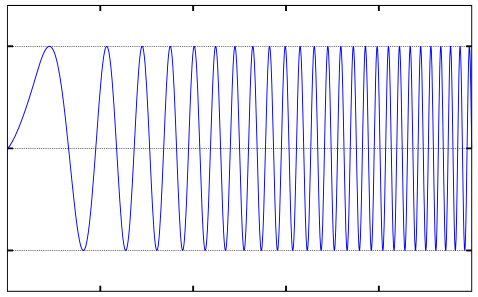
\includegraphics[width=.7\linewidth]{fig/lora_chirp.png}
\vspace*{5mm}
\caption{A CSS up-chirp. \cite{sghoslya_lora}}
\label{fig:lora_chirp}
\end{figure}

\subsection{Spreading factor}

The ratio between symbol and chirp rate is equal to $2$\textsuperscript{SF}. Spreading factor can take values between 7 to 12. Spreading factor also determines data rate of a LoRa transmission \cite{AN1200.22}. Comparison between various spreading factors can be seen in Figure \ref{fig:lora_sf_comparasion}. Spectrogram of an example LoRa transmission with various symbols can be found in Figure \ref{fig:lora_symbols}. Bit rate of a LoRa transmission can be calculated as:

\begin{equation} \label{eq:bit_rate_sf}
R_{b} = SF * \dfrac{\left[ \dfrac{4}{4+CR} \right] }{ \left[ \dfrac{2^{SF}}{BW|_{Hz}} \right]} * 1000 \ bps
\end{equation}

Where, $R_{b}$ is bit rate in bps, SF is spreading factor $SF \in \{7,..,12\}$, CR is error correction code rate $CR \in \{1,..,4\}$ and $BW$ is bandwidth in Hertz \cite{AN1200.22}. Bit rate for various spreading factors can be found in Table \ref{table:sf_data_rate}.

\begin{table}
\centering
\caption{Bit rate (bps) for various spreading factors (CR = 1).}
\label{table:sf_data_rate}
\begin{tabular}{|c|c|c|c|c|c|c|c|}
\hline
\multicolumn{2}{|c|}{\multirow{2}{*}{}} & \multicolumn{6}{c|}{\textbf{SF}} \\ \cline{3-8}
\multicolumn{2}{|c|}{}                  &    7 &    8 &    9 &   10 &   11 &   12 \\ \hline
\multirow{3}{*}{\textbf{BW (kHz)}}  & 125 & 5469 & 3125 & 1758 & 977 & 537 & 293 \\ \cline{2-8}
                                    & 250 & 10938 & 6250 & 3516 & 1953 & 1074 & 586 \\ \cline{2-8}
                                    & 500 & 21875 & 12500 & 7031 & 3906 & 2148 & 1172 \\ \hline
\end{tabular}
\end{table}

\begin{figure}
\centering
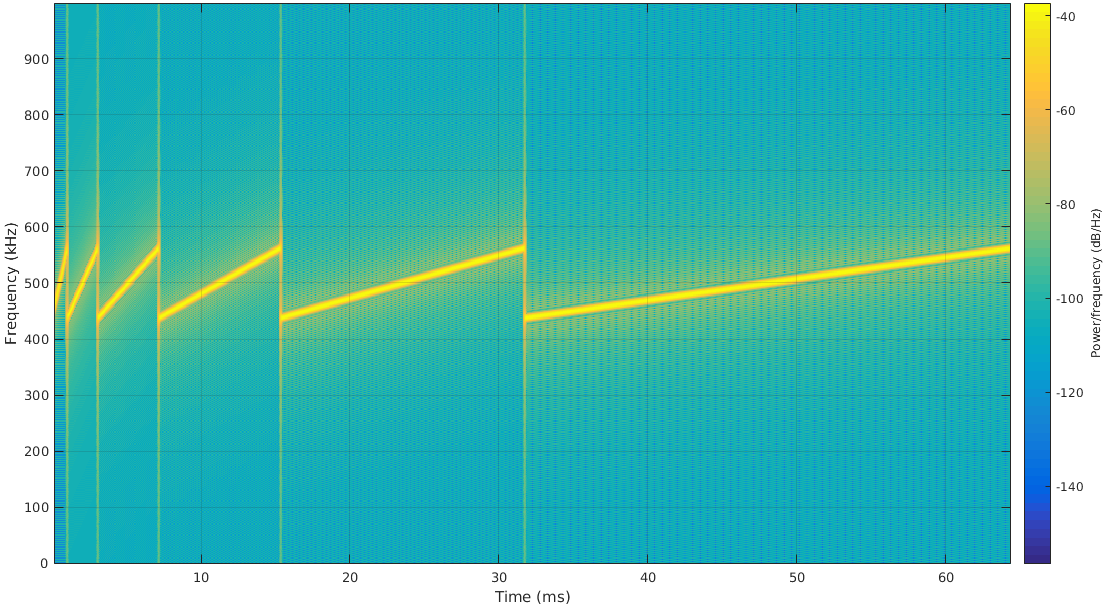
\includegraphics[width=.7\linewidth]{fig/lora_sf_comparasion.png}
\vspace*{4mm}
\caption{Spectrogram of various spreading factors (SF7 to SF12). \cite{sghoslya_lora}}
\label{fig:lora_sf_comparasion}
\end{figure}

\begin{figure}
\centering
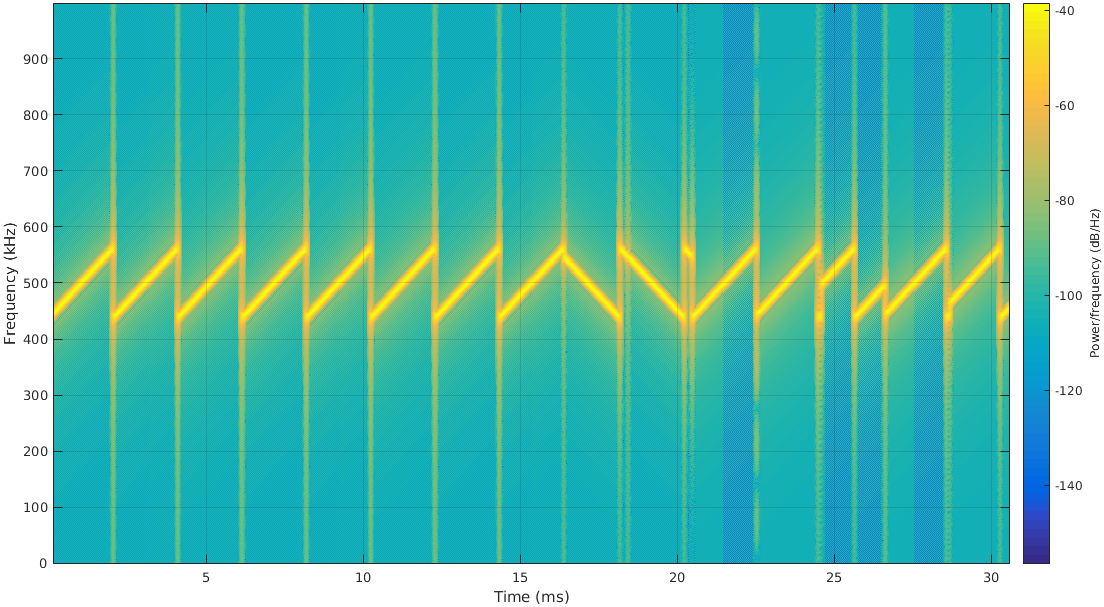
\includegraphics[width=.7\linewidth]{fig/lora_symbols.png}
\vspace*{4mm}
\caption{Spectrogram of an example LoRa transmission. \cite{sghoslya_lora}}
\label{fig:lora_symbols}
\end{figure}

When bandwidth and code rate are constant, as the spreading factor increases, the data rate decreases. Increasing the spreading factor makes the signal more resilient to noise thus increases the transmission range. Increasing the spreading factor also increases the transmission duration which increases the power consumption. Therefore, it is possible to trade between range and power consumption by changing spreading factor. Communication range of various spreading factors is roughly visualized in Figure \ref{fig:single_gw_empty}.

\begin{figure}
\centering
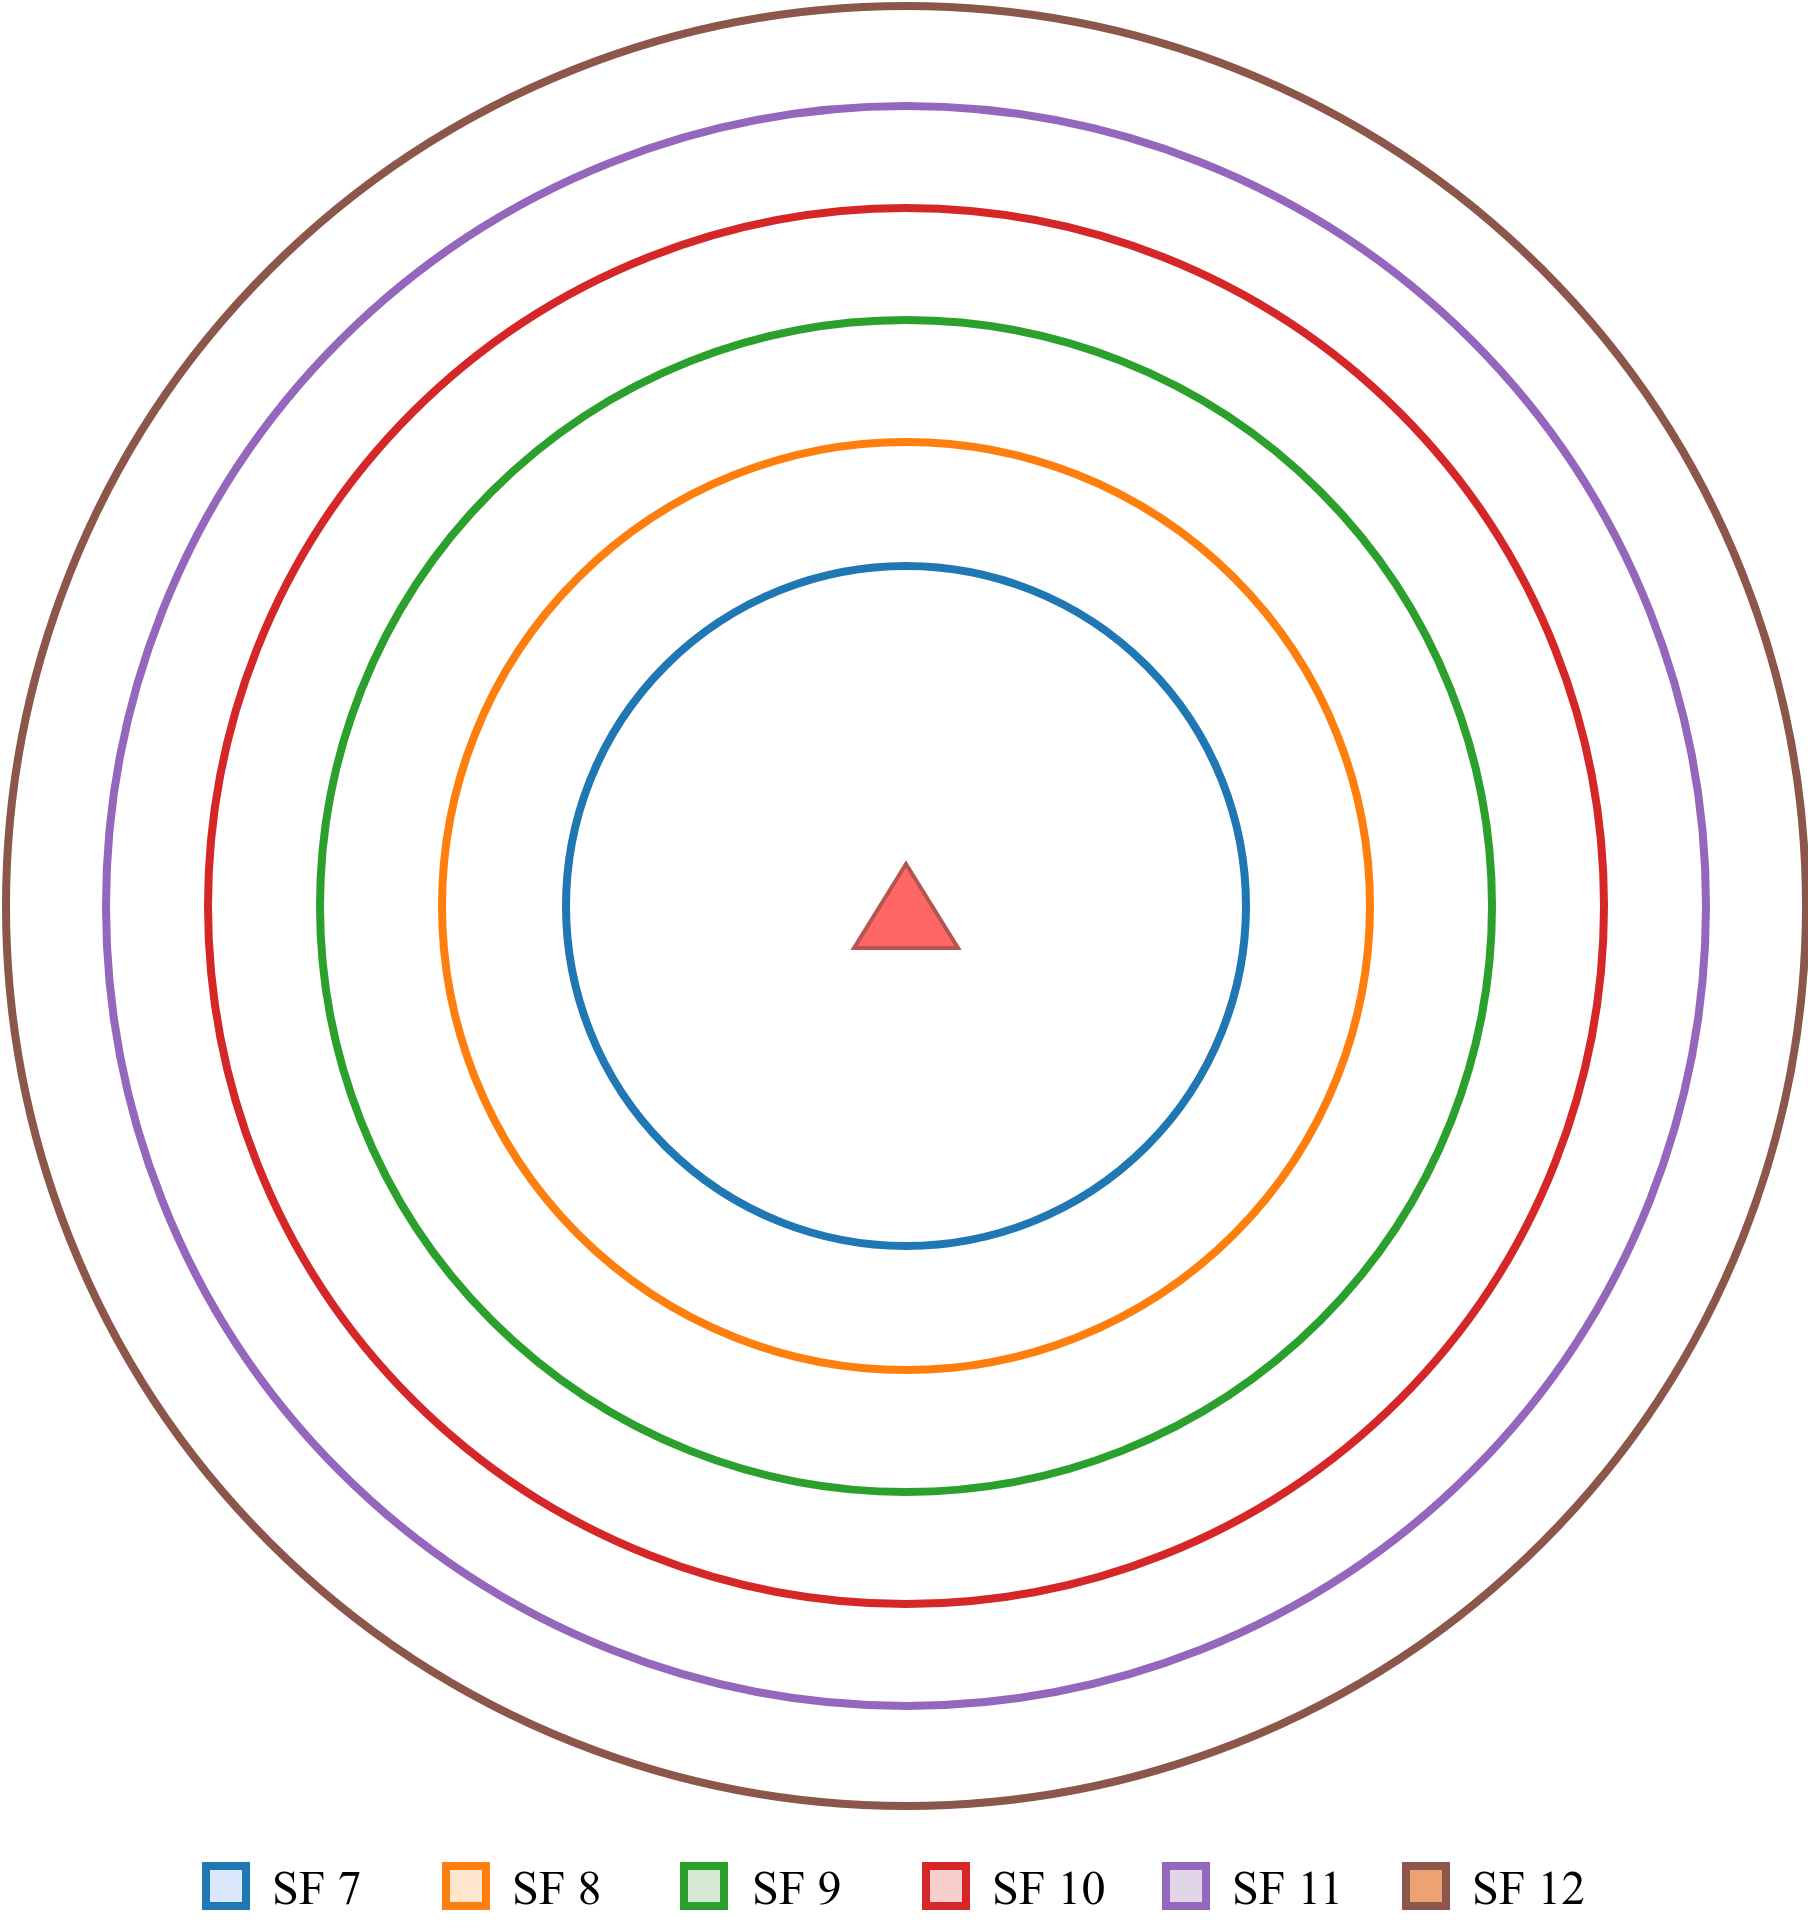
\includegraphics[width=.7\linewidth]{fig/lora_single_gw_empty.png}
\vspace*{5mm}
\caption{Various spreading factor communication (disproportionate) ranges.}
\label{fig:single_gw_empty}
\end{figure}

\subsection{Spreading factor assignment issue}

Simultaneous different spreading factor transmissions are orthogonal to each other up to some extent, which means that a LoRa gateway can simultaneously receive multiple transmissions with different spreading factors. However, simultaneous transmissions with the same spreading factor may not be received by the gateway due to collision. For this reason, spreading factor assignment of nodes is crucial for network performance \cite{8030482}.

In a LoRaWAN network, initially, a node is not aware of how far away it is from a gateway. However, a node can guess the distance from a gateway by observing received signal power of a downlink transmission. If received signal power of a downlink transmission is too high, then the node can decrease its next transmission spreading factor to decrease power consumption. This spreading factor assignment method is called lowest possible spreading factor assignment scheme for the rest of the thesis. Lowest possible spreading factor assignment scheme is commonly used in LoRaWAN deployments. Besides, gateway can request from a node to decrease its spreading factor or transmit power.

In Figure \ref{fig:collision}, a LoRaWAN network deployed with a single gateway is illustrated. Different color rings represent achievable range of different spreading factors from the gateway and different color circles represent selected spreading factor of the nodes. The end devices close to the gateway will fall into the lowest spreading factor (SF7) area section. The end devices close to the gateway will probably select the lowest spreading factor most of the time. This causes a lot of collisions between same spreading factor transmissions. Hence the number of collisions will increase as the number of end devices close to the gateway increases.

\begin{figure}
\centering
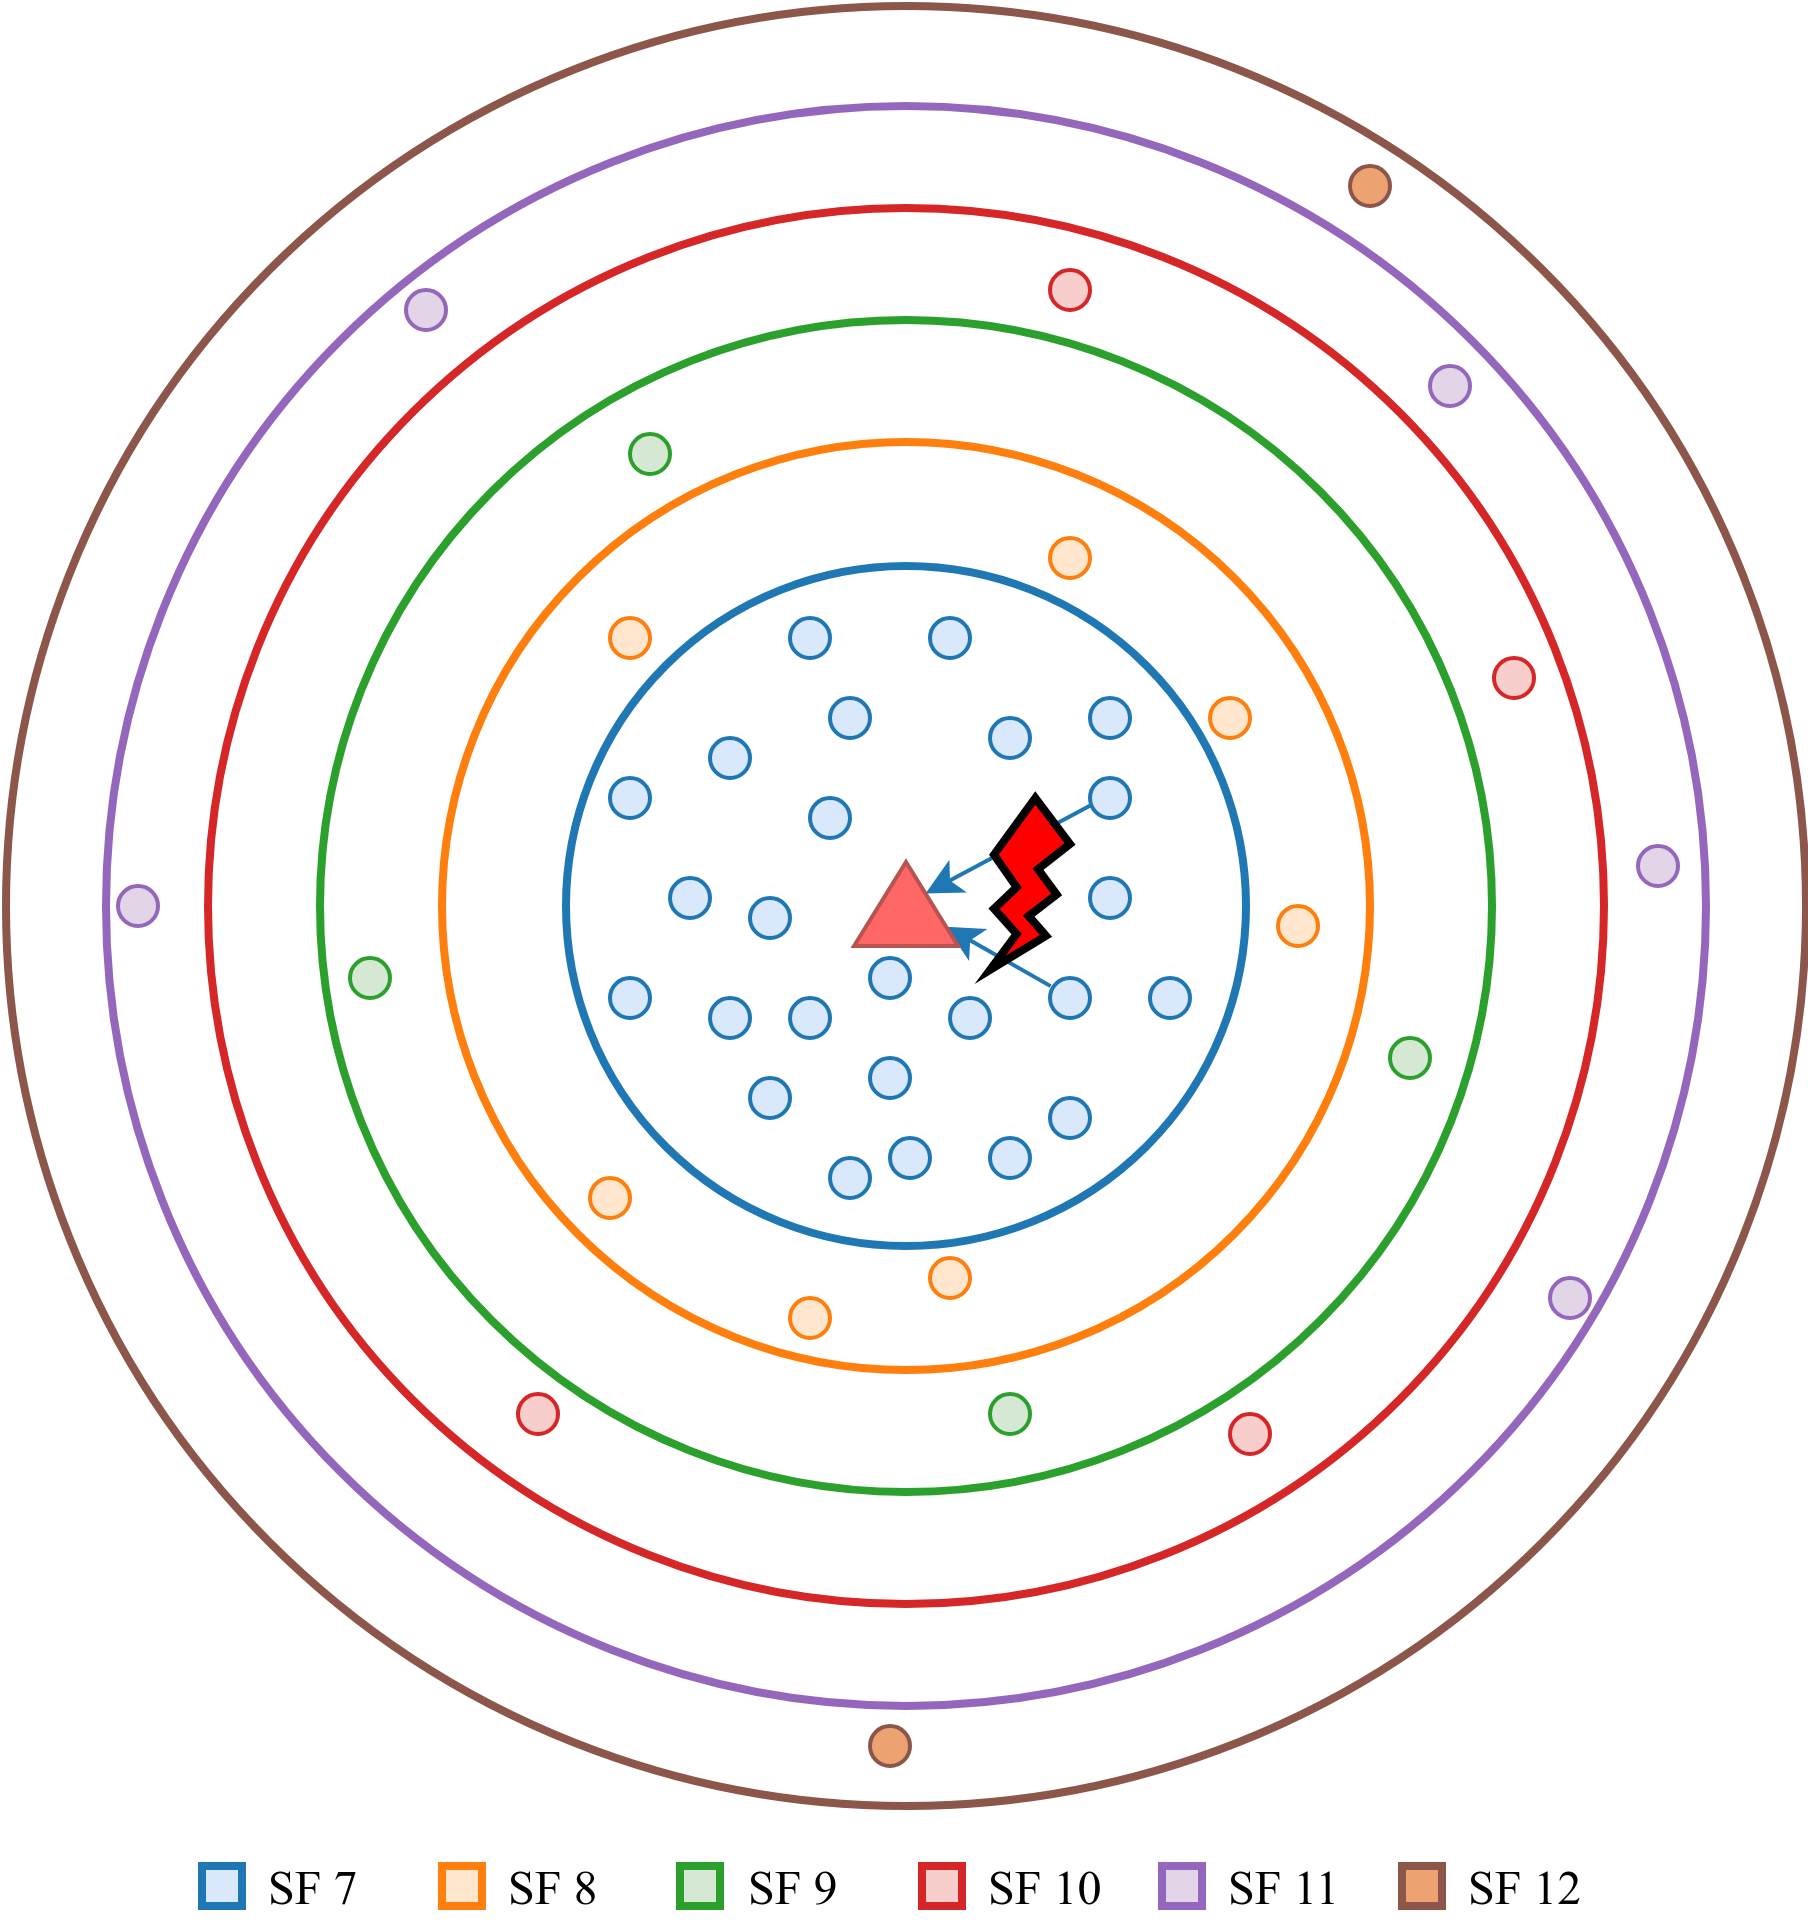
\includegraphics[width=.7\linewidth]{fig/lora_single_gw_collision.png}
\vspace*{5mm}
\caption{Collision between nodes close to the gateway.}
\label{fig:collision}
\end{figure}


\section{LoRaWAN}

LoRa has an open standard medium access control (MAC) layer protocol called LoRaWAN which is designed for large scale LoRa networks considering well known LPWAN challenges and their best practice solutions. LoRaWAN provides lightweight but powerful standard for wide range of LoRa IoT applications. LoRaWAN is developed and maintained by LoRa Alliance \cite{lora_alliance}. LoRa Alliance is an open, non-profit organization dedicated to standardization of LoRaWAN. LoRaWAN provides inter-operability between different LoRa networks. LoRa can be used as a wireless link technology without complying LoRaWAN, however this would break inter-operability between different LoRa networks. LoRaWAN is based on pure ALOHA medium access, which implies the end nodes do not check whether the channel is free or not before transmission, accepting the possibility of a collision. 

\subsection{Network structure}

A typical LoRaWAN network consists of three network entities, which are end node, gateway, and network server.

\subsubsection{End node}

LoRaWAN end node (EN) is a low power embedded device that only communicates with gateways. Single end node can communicate with multiple gateways. This communication architecture is called star of stars network topology. LoRaWAN star of stars network architecture is visualized in Figure \ref{fig:lorawan_topology}. LoRaWAN standard defines three classes for end devices which are Class A, Class B, and Class C. Different classes provide LPWAN solutions to different applications and deployments.

\begin{itemize}
  \item \textbf{Class A} end nodes generate uplink transmission at any time and only receive a period of time after uplink transmission (pure ALOHA manner). First receive window (Rx1) is opened after an uplink transmission at the same channel with uplink transmission. Then, second receive window (Rx2) is opened at different predefined channel. Transmit and receive windows timing diagram can be found in Figure \ref{fig:lorawan_class}. Class A offers lowest energy consumption. Class A behavior is the default operation mode of LoRaWAN end devices.
  \item \textbf{Class B} end nodes extend Class A behavior by adding scheduled periodic receive windows (Rx2). Receive window is synchronized using a beacon packet transmitted by gateways.
  \item \textbf{Class C} end nodes extend Class A behavior by keeping receive window (Rx2) open all the time except uplink transmission duration. This provides Class C end nodes with low latency downlink communication, which requires more power consumption. Thus, Class C is suitable for applications which are delay intolerant and end devices which are connected to power grid.
\end{itemize}

\begin{figure}
\centering
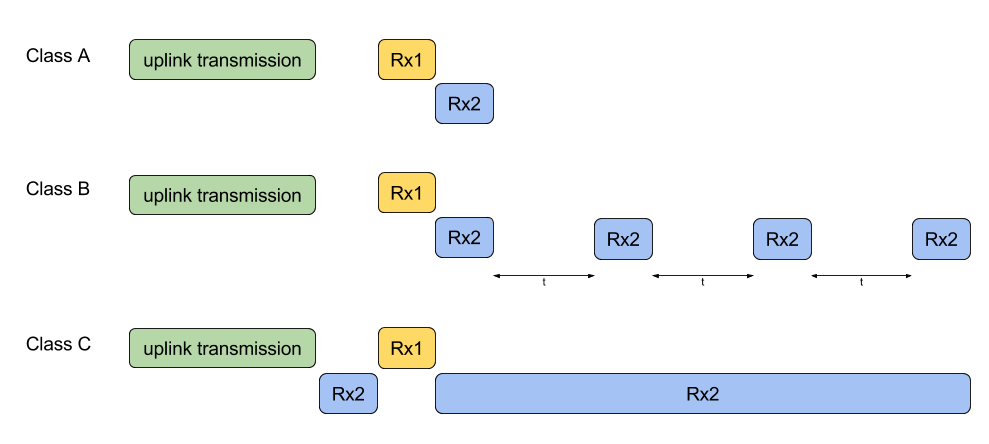
\includegraphics[width=\linewidth]{fig/lorawan_class.png}
\vspace*{4mm}
\caption{LoRaWAN class A, B and C TX/RX timing diagram \cite{witekio}.}
\label{fig:lorawan_class}
\end{figure}

In this thesis, only Class A end devices are considered since Class A behavior leads to the lowest power consumption and Class A is the default operation mode.

\newpage

\subsubsection{Gateway}

LoRaWAN gateway (GW) is a device that receive/transmit packets coming from/to end nodes. A typical gateway can receive from multiple channels at the same time. Gateways are usually connected to power grid, so power consumption of a gateway is insignificant in most of the deployments.

\subsubsection{Network server}

LoRaWAN network server (NS) is a server that provides MAC layer processing. Network server routes messages from application to end nodes and vice versa. Network server can be used for tweaking end node parameters such as channel, transmit power and spreading factor to increase network performance. NS is the brain of the LoRaWAN network. All process hungry calculations and applications can be run in NS. For example, NS can locate end node locations by triangulation if an uplink transmission is received by at least 3 gateways.

\begin{figure}
\centering
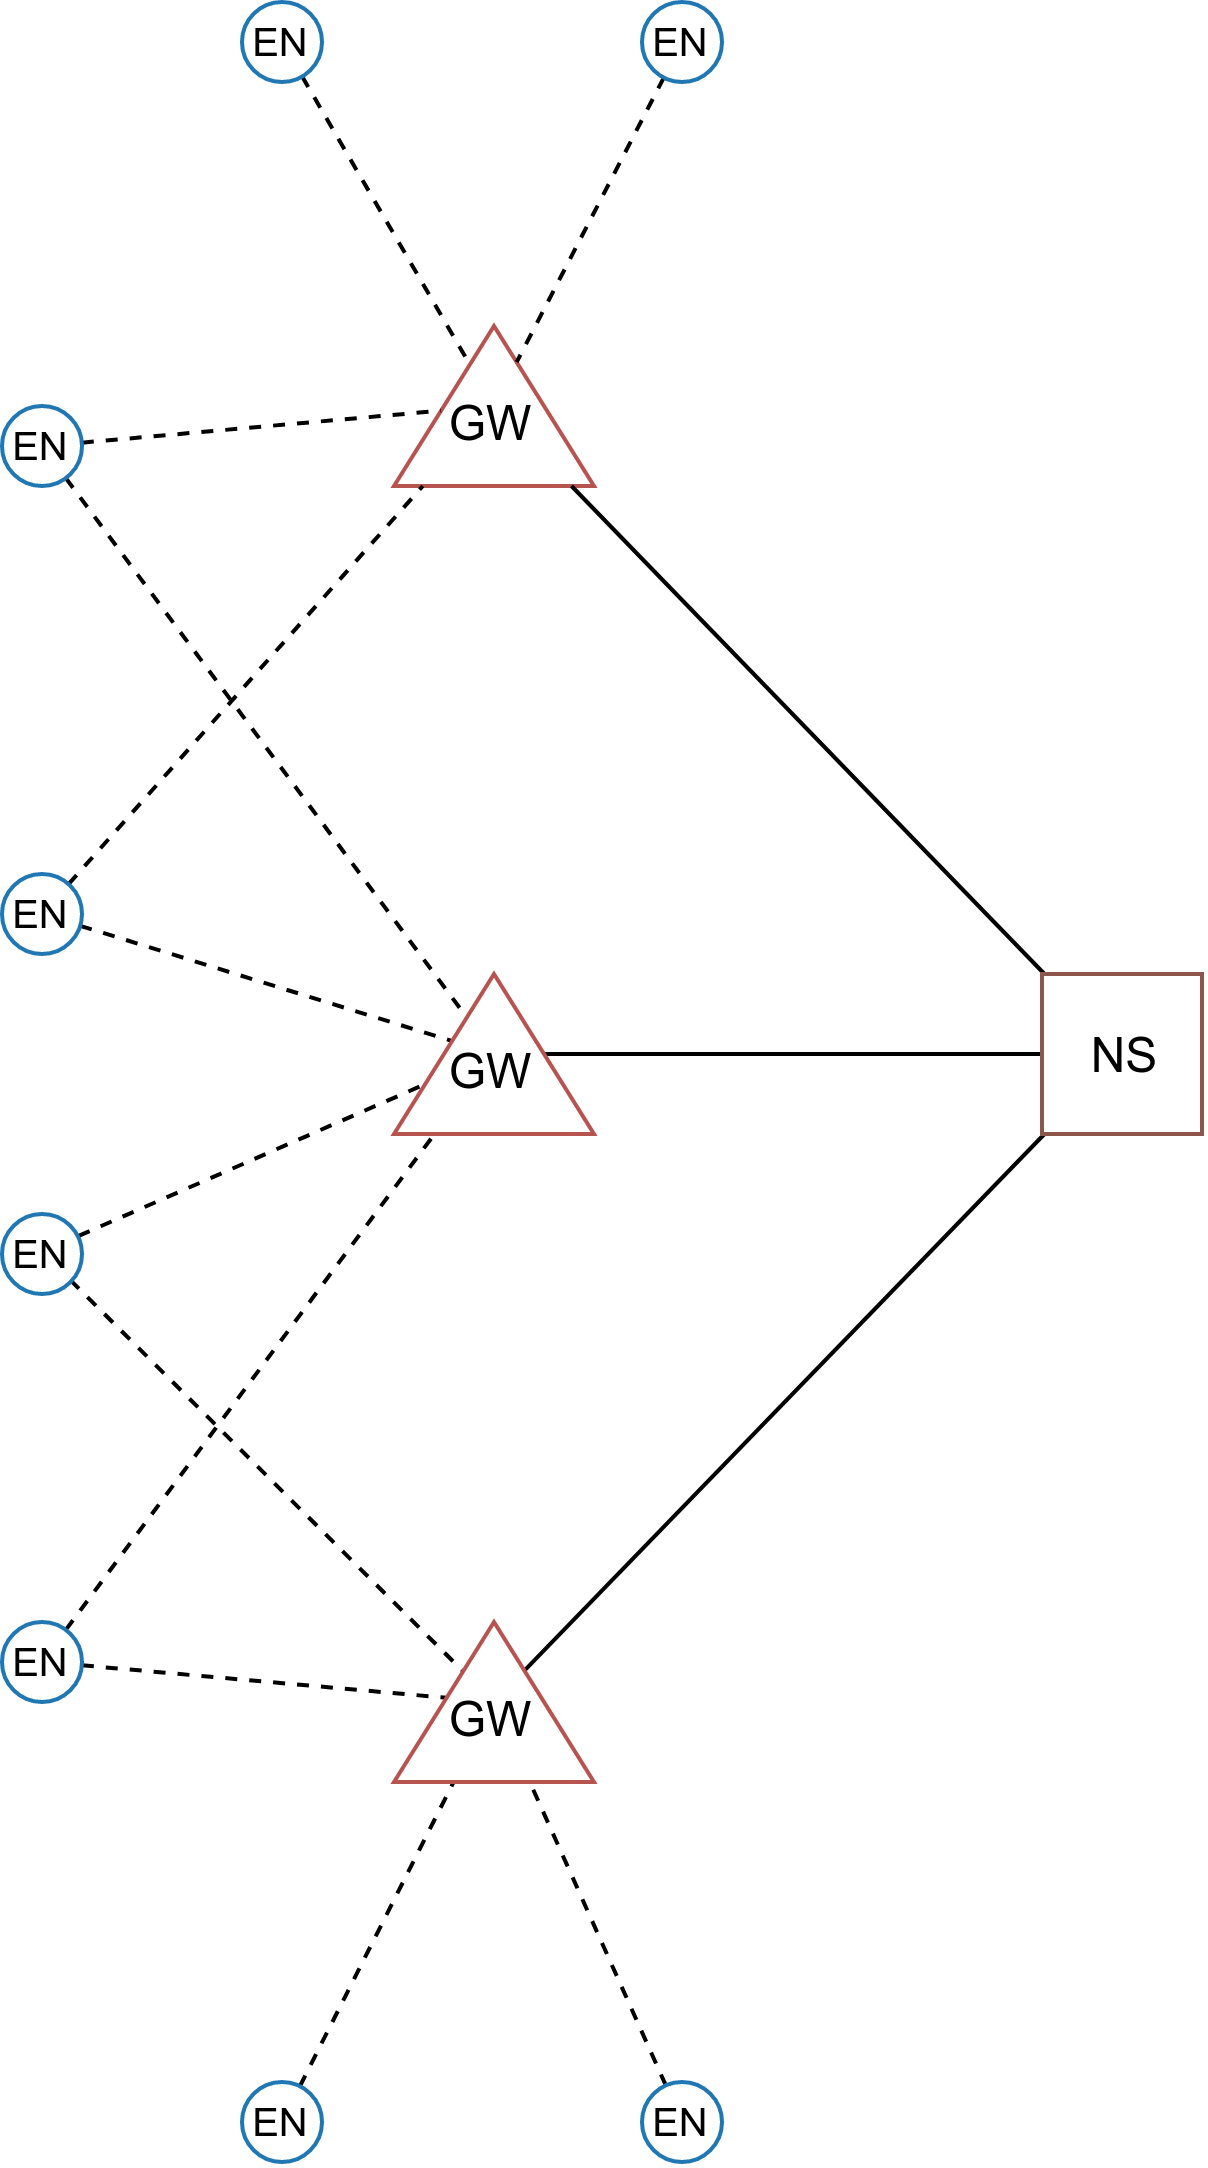
\includegraphics[width=.7\linewidth]{fig/lorawan_topology.png}
\vspace*{4mm}
\caption{LoRaWAN star of stars network architecture.}
\label{fig:lorawan_topology}
\end{figure}

\subsection{Packet structure}
LoRaWAN specification describes the communication protocol and packaging format. LoRaWAN PHY and MAC layer packet structures can be seen in Figure \ref{fig:lorawan_mac}. PHY layer packet consist of a preamble, a header, a header CRC, a payload and a payload CRC. The MAC payload consists of a frame header, a frame port and a frame payload. The frame header consists of a device address, a frame control field, a frame counter and a frame option field. Frame control field is used for Adaptive Data Rate (ADR) feature. NS is able to ask to an end node to modify spreading factor. If ADR bit in the frame control field is set, then spreading factor of the end node's future transmissions are controlled by the NS. NS provides new spreading factor information in frame options field \cite{lorawan.specification}. The ADR algorithm is not standardized in LoRaWAN protocol. ADR implementation is left to the network operators. If ADR feature is enabled in a network, then the ADR algorithm should select a spreading factor which is high enough to provide a reliable link and low enough to minimize transmission time to avoid collisions.

\begin{figure}
\centering
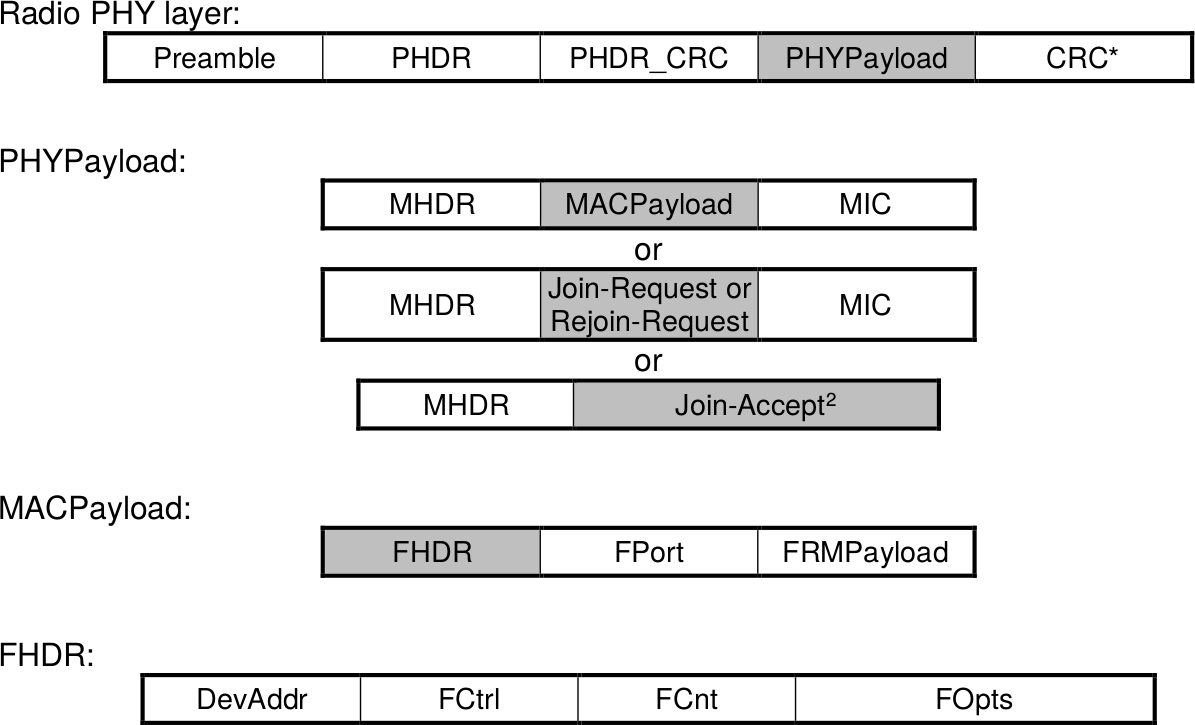
\includegraphics[width=\linewidth]{fig/lorawan_mac.png}
\vspace*{4mm}
\caption{LoRaWAN packet format \cite{lorawan.specification}.}
\label{fig:lorawan_mac}
\end{figure}


\section{ISM Band Regulations}
LoRaWAN operates in license free Industrial, Scientific, and Medical (ISM) bands. It operates in 902-928 MHz in US and 863-870 MHz in Europe \cite{lorawan.regional.parameters}. ISM bands are subject to radio transmission time regulations to prevent any device to occupy the channel too long. So, transmissions are required to either adopt listen before talk policy or duty cycle restrictions. Most of the LPWAN technologies adopt duty cycle restrictions since listen before talk policy requires much more power consumption. LoRaWAN obeys duty cycle restrictions. Also, ISM bands are subject to effective isotropic radiated power (EIRP) restrictions. For the rest of this thesis, European ISM band regulations are considered.

\begin{itemize}
  \item \textbf{Duty Cycle Restriction} is a limitation on percentage of air time. For example, 1\% duty cycle restriction enforces a device such that single transmission cannot exceed 3.6 seconds and total time on air in one hour cannot exceed 36 seconds. Duty cycle limitations for various European ISM channels can be found in Table \ref{table:max_tx_power}. This limitation is applied for every radio device who don't adopt listen before talk policy. This includes all LoRaWAN end nodes and gateways.
  \item \textbf{Effective Isotropic Radiated Power Restriction} sets maximum allowed transmit power of a transmitter. Maximum allowed effective radiated power for various European ISM channels can be found in Table \ref{table:max_tx_power}.
\end{itemize}

\begin{table}[h]
\centering
\caption{EU863-870 ISM band LoRa channels \cite{EN300.220} \cite{lorawan.regional.parameters}.}
\label{table:max_tx_power}
\begin{tabular}{|c|c|c|c|}
\hline
\textbf{Frequency (MHz)} & \textbf{Bandwidth (kHz)} & \textbf{Max Duty Cycle (\%)} & \textbf{Max ERP (dBm)} \\ \hline
      863.0 - 868.0  &   125 &   1   &   14 \\ \hline
      868.0 - 868.6  &   125 &   1   &   14 \\ \hline
      868.7 - 869.2  &   125 &   0.1 &   14 \\ \hline
      869.4 - 869.65 &   125 &   10  &   14 \\ \hline
      869.7 - 870.0  &   125 &   1   &   14 \\ \hline
\end{tabular}
\end{table}
